% ##############################################################################
% ##############################################################################
% #######   PLANTILLA FODAMI CAIM-CAIFE 2025                            ######## 
% #######   Creado con TeXstudio v 4.8.6   (c/archivo .cls)             ########
% #######   Autores: Equipo FIE - EAS|EAH|SEM                           ########
% ##############################################################################
\documentclass[a4paper]{fodami}        % customizado en archivo .cls    ########
%\usepackage{showframe}                % show layout de página (opt)    ########
% ##############################################################################
% ##############################################################################

% ---------- TÍTULO ------------------------------------------------------------
\title{\textbf{INTRODUCCIÓN TEMPRANA DE LA MECÁNICA COMPUTACIONAL EN CURSOS DE ELECTROSTÁTICA Y MECÁNICA ANALÍTICA}}

% ---------- AUTORES -----------------------------------------------------------
\author[1*]  {\textbf{Nombre A. Apellido}}
\author[2,3]{\textbf{Nombre B. Apellido}}
\author[4]{\textbf{Edgardo Palazzo}}

% ---------- AFILIACIÓN --------------------------------------------------------
\setlength\parindent{0pt}
\affil[1]{Departamento Académico de Mecánica, UTN - Facultad Regional Santa Fe, Lavaisse 610, 3000 Santa Fe, Argentina.}

\affil[2]{CONICET,Instituto ............................... }

\affil[3]{Facultad de Ingeniería, Universidad ...... }

\affil[4]{Departamento de Materias Básicas, UTN - Facultad Regional Avellaneda, Ramón Franco 5050, B1876ABY Villa Domínico, Buenos Aires, Argentina}

\affil[*]{Email: autor.de.contacto@ ......... (en color negro y sin subrayar)}



% ##############################################################################
\begin{document}
\date{}

% ########## ENCABEZAMIENTOS y PIE #############################################
\renewcommand{\headrulewidth}{0pt} \renewcommand{\footrulewidth}{0pt}
\pagestyle{fancy}
\fancyhead{}
\fancyhead[C]{
	
\includegraphics[width=11.5cm]{imagenes/logoFODAMICAIMCAIFE.pdf}
	\noindent
	{\color{lightgray} \rule{\linewidth}{0.14cm}}
}
\fancyfoot{}
\fancyfootoffset[L]{-4cm}
\fancyfoot[L]{\footnotesize \flushleft \emph{IX CAIM 2025 - Noveno Congreso Argentino de Ingeniería Mecánica \\  
	IV CAIFE 2025 - Cuarto Congreso Argentino de Ingeniería Ferroviaria} \\
	\url{www.fie.undef.edu.ar/caimcaife2025} |  \href{mailto:caimcaife2025@fie.undef.edu.ar}{caimcaife2025@fie.undef.edu.ar}}
\setlength{\parskip}{8pt}
% ##############################################################################
	
\maketitle
\thispagestyle{fancy}

% ---------- RESUMEN -----------------------------------------------------------
\section*{
	\begin{center}
		RESUMEN
	\end{center}}
\vspace{-1.0cm}
Este documento debe utilizarse como plantilla para el trabajo completo a presentar en el IX Congreso Argentino de Ingeniería Mecánica / IV Congreso Argentino de Ingeniería Ferroviaria. Contiene la estructura y formatos de texto.\\
La primera página solo debe contener el Título, los Autores (hasta 6), la filiación, el Resumen y las Palabras clave. \textbf{El TÍTULO DEL TRABAJO}, en letra Arial 12 Mayúsculas Negrita, centrado, distanciado del encabezado por cuatro renglones de 12 pts. Con un renglón de separación se incluyen los autores del trabajo, identificados con el primer nombre, la inicial del segundo nombre y el apellido, en \textbf{ARIAL 10 negrita} centrados. Si la cantidad de autores ocupa mas de un renglón, entre ellos interlineado sencillo, y el último renglón con espaciado posterior 6pt. A continuación, en el renglón siguiente se indican las instituciones de los autores, sin repetirlas y con las correspondientes direcciones postales (en Arial 10) referidas con superíndices numéricos en los Apellidos. En el reglón siguiente, se debe indicar el e-mail del “autor de contacto” indicado con superíndice asterisco “*” en el listado de autores. \\
Luego debe ir centrada la palabra \textbf{RESUMEN}, en Arial 10 negrita mayúscula, con un espaciado anterior de 24 pt y posterior de 6 pt. 
El texto del resumen se escribe en Arial 10, con interlineado sencillo, sin espaciado entre párrafos, y alineación justificada. El mismo deberá contener el objetivo del trabajo, la metodología, resultados y conclusiones, sin superar las 300 palabras. En el trabajo completo, el resumen podrá tener diferencias respecto del aceptado originalmente, en la medida que no altere la naturaleza del objetivo del trabajo. \\
A continuación, dejando un espacio de (10 pt.), se deben incluir las palabras clave, hasta un máximo de cuatro (4), en Arial 10 cursiva, con la primera letra de cada palabra en mayúscula.


\textit{\textbf{Palabras claves}: Formato Trabajo; Congreso; Ingeniería Mecánica; Ingeniería Ferroviaria.}
	
% ---------- CUERPO del DOCUMENTO ----------------------------------------------
\newpage
\onehalfspacing
\setlength{\parskip}{0pt}
% ------------------------------------------------------------------------------
\section{INTRODUCCIÓN}
La segunda página comenzará con el título \textbf{1. INTRODUCCIÓN}. El cuerpo del artículo, se escribirá en ARIAL 10 con interlineado 1.5. Todos los títulos y textos en color negro. \\ 
Los trabajos serán evaluados por el Comité Técnico Científico (CTC) considerando:
\begin{itemize}
	\item \textbf{Formato}: El mismo debe cumplir con las normas de presentación establecidas, incluyendo estructura, estilo y formato específico solicitado. 
	\item \textbf{Correspondencia de título y resumen con el trabajo completo}: El título y el resumen deben reflejar el contenido del trabajo completo.
	\item \textbf{Consistencia gramatical e idiomática}: El trabajo debe redactarse con un lenguaje claro, preciso y formal, libre de errores gramaticales, ortográficos o de puntuación y con coherencia en los párrafos escritos. 
	\item \textbf{Introducción}: Se debe presentar un contexto significativo del estudio o investigación, detallando el planteo del problema y definiendo los objetivos y los alcances del trabajo.
	\item \textbf{Descripción de la metodología}: Se debe detallar de manera precisa el enfoque, los métodos y las herramientas utilizadas para el desarrollo del estudio o investigación.  
	\item \textbf{Resultados}: Se deben presentar los hallazgos de manera organizada, respaldados por datos y análisis pertinentes. Relación de los resultados con los objetivos planteados. Explicación de patrones o tendencias observadas.
	\item \textbf{Conclusiones}: Se deben incluir los resultados más importantes, destacando la relevancia de los mismos y sus posibles implicaciones.
	\item \textbf{Referencias y bibliografía}: Se deben incorporar las fuentes consultadas, siguiendo el formato de citación indicado en el documento. Las referencias deben ser relevantes, actuales y apropiadas para el tema tratado.
\end{itemize}
Los trabajos deben tener una extensión mínima de 6 (seis) páginas y máxima 12 (doce) páginas. Los autores NO deben numerar las páginas del documento. Las notas a pie de página deberán ser completamente evitadas. Si se utilizan acrónimos, deben ser definidos inmediatamente antes de su primera ocurrencia. \\
Los trabajos serán elevados mediante el procedimiento indicado en la página Web del Congreso a través del OCS (Open Conference System). Se notificará a los autores el resultado de la evaluación en el plazo especificado. Los trabajos aprobados, cuyos autores hayan acreditado la matrícula de inscripción, se publicarán en las Actas del Congreso, las que se pondrán a disposición de los autores por procedimiento ad-hoc. El número máximo de autores por trabajo es 6 (seis). \\
Para participar en las actividades del IX CAIM / IV CAIFE 2025 se debe abonar la matrícula de inscripción como autor o asistente. La “matrícula de autor”, otorga el derecho a exponer hasta dos (2) trabajos y que los mismos sean incluidos en las actas del congreso. La exposición oral solo podrá ser realizada por alguno de los autores del trabajo, que haya abonado la matrícula de inscripción. \\
Se procurará maximizar el número de ponencias orales de manera de favorecer la discusión y el intercambio de ideas entre participantes. Asimismo, para autores que presenten más de un trabajo, uno de ellos, a juicio del CTC y de la Organización, podrá ser seleccionado para ser presentado mediante poster \\
El español es el idioma oficial del Congreso. También se podrán presentar trabajos en portugués y en inglés. \\
Los trabajos serán enviados en formato digital PDF, pudiendo contener gráficos y/o figuras en color. El tamaño de página será el correspondiente al formato A4 (210 x 297 mm), con márgenes de 4 cm superior (que corresponden al encabezado de las páginas con el logo del congreso), 2 cm inferior (que corresponde al pie de página) y 2.5 cm izquierdo y derecho. Por consultas sobre envíos de trabajos al OCS escribir a: \href{mailto:caimcaife.mesadeayuda@gmail.com}{caimcaife.mesadeayuda@gmail.com} \\
En lo que se refiere a su estructura, el trabajo se dividirá en secciones, numeradas en orden ascendente y titulado en \textbf{ARIAL 10, negrita}. Según el contenido y la temática de los trabajos, puedan contemplarse diferentes secciones; se recomienda en general, seguir una estructura clásica con una introducción, en la que se incluyan los antecedentes y objetivos del trabajo, una parte analítica y/o experimental en la que se describan los procedimientos, equipos y métodos, una sección dedicada a presentar y discutir los resultados, una sección en la que se relacionen las principales conclusiones del trabajo y una última sección dedicada a las referencias bibliográficas.\\
En relación con esto último, las referencias bibliográficas, se indicarán en el texto entre corchetes, numeradas por orden de aparición en el mismo, en la forma [1], y se incluirán al final del texto (ver sección 4). Para más de una referencia, debe usarse [1,3] (referencias 1 y 3) y [2-4] (referencias 2,3 y 4). Adicionalmente, puede incluirse una sección dedicada a los agradecimientos a personas o instituciones que han contribuido para la realización y/o financiación del trabajo.

\subsection{Subsecciones}
Cada sección puede quedar dividida en diferentes subsecciones que se numerarán en orden ascendente mediante dos números, el primero indicativo de la sección y el segundo de la subsección correspondiente. Cada título de subsección, en \textbf{ARIAL 10, negrita}, primera letra mayúscula, tendrá espaciado anterior 12 pt. y espaciado posterior 6 pt.  A su vez, una subsección puede dividirse en apartados, 

\subsubsection{Apartado en una subsección}
Éste es un ejemplo de apartado dentro de una subsección, \textbf{con el título del apartado, en Arial 10 negrita cursiva}, con espaciado anterior 12 pt. y espaciado posterior 3 pt. 

\subsubsection{Formato electrónico y envío de los trabajos}
Los trabajos, deberán subirse a la plataforma de autogestión (OCS), únicamente en PDF, respetando el formato indicado en este documento, hasta la fecha límite para la presentación de trabajos publicada en la página Web del Congreso.\\
Se puede acceder al OCS directamente en \url{https://amcaonline.org.ar/caim-caife} o desde la página Web del congreso: \url{https://www.caimcaife2025@fie.undef.edu.ar}

% ------------------------------------------------------------------------------
\section{ECUACIONES, FIGURAS Y TABLAS}
Cada ecuación debe estar numerada utilizando números arábigos entre paréntesis. Las ecuaciones en ARIAL 10, se insertarán en líneas independientes del texto, irán centradas, dejando un espacio de 6pt arriba y abajo para separarla del texto que la rodea. Se referirán en el texto mediante Ecuación (1), Ecuación (2).
\begin{equation}\label{eq:primera}
	F(t)=at^{-n}
\end{equation}
Se recomienda priorizar el uso del Sistema Internacional de Unidades (S.I.). \\
Las figuras se insertarán, de forma que queden independientes del texto, centradas, y con una leyenda inferior, escrita en ARIAL 10, tal y como se indica en el ejemplo de la Figura 1. Deberán estar numeradas consecutivamente en el orden en el que aparezcan. Las Figuras deberán estar separadas, un renglón de 10 pt de los párrafos anterior y posterior a la misma. \\
En el cuerpo del texto se referirán mediante la palabra Figura seguida del número correspondiente.
\begin{figure}[h]
	\centering
	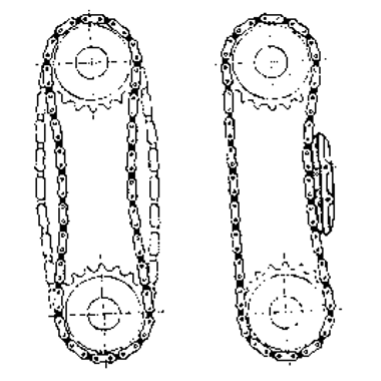
\includegraphics[width=43mm]{imagenes/figura1.png}
	\caption{Ejemplo de figura inserta en texto.}
	\label{fig:cadenas}
\end{figure} \\
Las Tablas se insertarán, de forma que queden independientes del texto, centradas, y con una leyenda superior, escrita en ARIAL 10, tal y como se indica en el ejemplo de la Tabla 1:
\begin{table}[h]
	\centering
	\setlength{\tabcolsep}{36pt}
	\renewcommand{\arraystretch}{1.3}
	\caption{Ejemplo de tabla inserta en texto }
	\begin{tabular}{ |c|c|c| }
		\hline
		Parámetros & $\cdots$  & $\cdots$ \\
		\hline \hline
		$Z_1$      &           &          \\
		\hline
		$Z_2$      &           &          \\
		\hline	
	\end{tabular}
	\label{table:data}
\end{table} \\
Todas las tablas deben estar numeradas. En el texto se hará referencia a las mismas mediante la palabra Tabla seguida del número de orden en el que aparezcan. Las Tablas deberán estar separadas, un renglón de 10 pt de los párrafos anterior y posterior a la misma.
% ------------------------------------------------------------------------------
\section{CONCLUSIONES}
Se apreciará que las mismas evidencien solidez y coherencia. Pueden incluirse en ellas otras cuestiones, como, por ejemplo, mención de interrogantes no dilucidados que podrían ser abordados en el futuro.

% ------------------------------------------------------------------------------
\section{AGRADECIMIENTOS}
Adicionalmente, puede incluirse un apartado dedicado a los agradecimientos a personas o instituciones que han contribuido para la realización y/o financiación del trabajo.

Los autores de este trabajo desean agradecer a …… por el apoyo …………….
% -----------------------------------------------------------------------------	
\section{REFERENCIAS}
Se considera valioso incluir menciones a textos y artículos de publicaciones reconocidas, valorándose la incorporación de aquellas de reciente edición. La forma de indicar las citas bibliográficas en el texto está especificada al final de la sección \textbf{1. INTRODUCCIÓN}. Solamente deben incluirse las referencias citadas en el cuerpo del documento, según su orden de aparición. El formato de las referencias según \textbf{Normas APA (7ª edición, 2024)}. A continuación, se brindan algunos ejemplos:

\textbf{1. Libro} \cite{budynas_diseno_2012}

[1] Apellido, A. A. y Apellido, B.B. (Año). Título del libro en cursiva. Edición. Editorial.

\textit{\textbf{Ejemplo:}}
\begin{enumerate}[label={[}\arabic*{]}]
	\item Budynas, R.G. and Nisbett, J. K.  (2012). \textit{Shigley's Mechanical Engineering Design}. 9th Ed. McGraw-Hill.
\end{enumerate}

\textbf{2. Artículo de revista} \cite{moreno_abandono_2019}

[2] Apellido, A.A. y Apellido, B.B. (Año). Título del artículo. Título de la revista en cursiva, volumen(número), páginas. https://doi.org/xxxx (si está disponible).

\textit{\textbf{Ejemplo:}}
\begin{enumerate}[label={[}\arabic*{]}]
	\setcounter{enumi}{1}
	\item Moreno J. and Chiecher A., (2019). \textit{Dropout in Engineering careers. A study of academic, socio-demographic, labor and life aspects}. Educational Research Notebooks, 10, (2),73-90, DOI:\\ https://doi.org/10.18861/cied.2019.10.2.2908
\end{enumerate}


\textbf{3. Artículo en línea} \cite{lu_aprobarias_2015}

[3] Apellido, A. A. (Año). Título del artículo. Nombre del sitio web. URL

\textit{\textbf{Ejemplo:}}
\begin{enumerate}[label={[}\arabic*{]}]
	\setcounter{enumi}{2}
	\item Lu S. and Whiteman H. (2015) \textit{¿Would you pass the college entrance exam in China?}, CNN in espanish.\\
	https://cnnespanol.cnn.com/2015/06/09/aprobarias-el-examen-de-ingreso-a-la-universidad-en-china
\end{enumerate}

\textbf{4. Informe o documento institucional} \cite{organizacion_mundial_de_la_salud_informe_2020}

[4] Nombre de la institución. (Año). Título del informe en cursiva. URL (si aplica)

\textit{\textbf{Ejemplo:}}
\begin{enumerate}[label={[}\arabic*{]}]
	\setcounter{enumi}{3}
	\item World Health Organization. (2020). \textit{The World Mental Health Report}.\\
	https://www.who.int/informes/saludmental2020
\end{enumerate}

\textbf{5. Tesis o disertación} \cite{jerez_resultados_2012}

[5] Apellido, A. A. (Año). Título de la tesis o disertación en cursiva (Tesis doctoral, Nombre de la Institución que otorga el título). Nombre de la base de datos. URL (si está disponible)

\textit{\textbf{Ejemplo:}}
\begin{enumerate}[label={[}\arabic*{]}]
	\setcounter{enumi}{4}
	\item Jerez, O., (2012), \textit{Los resultados de aprendizaje en la Educación Superior por Competencias}. Doctoral Thesis, University of Granada, Spain. ISSN: 978-84-695.1027-8. https://dialnet.unirioja.es/servlet/tesis?codigo=62470
\end{enumerate}

\textbf{6. Norma o estándar} \cite{noauthor_iso_2020}

[6] Nombre del organismo. (Año). Título de la norma en cursiva (Código y número de la norma). Editorial (si aplica). URL (si se obtuvo en línea).

\textit{\textbf{Ejemplo:}}
\begin{enumerate}[label={[}\arabic*{]}]
	\setcounter{enumi}{5}
	\item International Organization for Standardization. (2020). ISO 9001:2015: \textit{Sistemas de gestión de la calidad (Norma Internacional 9001)}.
\end{enumerate}	

\textbf{7. Trabajo presentado en un congreso o conferencia} \cite{xiaobin_stress_2013}

[7] Apellido, A. A., y Apellido, N. T. (Año). Título del trabajo. Denominación del Congreso, Registro (ISBN o ISSN), Lugar y fechas.

\textit{\textbf{Ejemplo:}}
\begin{enumerate}[label={[}\arabic*{]}]
	\setcounter{enumi}{6}
	\item Xiaobin L. y Zelong L. (2013). \textit{Stress concentration factors due to typical geometric discontinuities for shaft design by numerical simulation}. ASEE Annual Conference and Exposition, Atlanta, Georgia, June 23-26, 2013, DOI 10.18260/1-2—22476 
\end{enumerate}

{\color{gray} \rule{\linewidth}{0.5pt}}
\textbf{Pautas importantes:}
\begin{itemize}
	\item \textbf{Cursiva}: Los títulos de libros y de revistas, denominación de congreso y normas deben ir en cursiva.
	\item \textbf{DOI}: Si un artículo tiene un DOI, debe incluirse al final de la referencia.
	\item \textbf{URL}: En el caso de las fuentes en línea, incluye la URL completa, con texto en color negro sin formato de hipervínculo. No aplica ``Recuperado de'' a menos que sea necesario (por ejemplo, si la fecha de acceso es relevante).
\end{itemize}

% ------------------------------------------------------------------------------
\renewcommand{\bibname}{Referencias}% cambio de nombre
\nocite{*}
%\printbibliography
	
\end{document}

% ##############################################################################
% ##############################################################################
